\documentclass[1p]{elsarticle_modified}
%\bibliographystyle{elsarticle-num}

%\usepackage[colorlinks]{hyperref}
%\usepackage{abbrmath_seonhwa} %\Abb, \Ascr, \Acal ,\Abf, \Afrak
\usepackage{amsfonts}
\usepackage{amssymb}
\usepackage{amsmath}
\usepackage{amsthm}
\usepackage{scalefnt}
\usepackage{amsbsy}
\usepackage{kotex}
\usepackage{caption}
\usepackage{subfig}
\usepackage{color}
\usepackage{graphicx}
\usepackage{xcolor} %% white, black, red, green, blue, cyan, magenta, yellow
\usepackage{float}
\usepackage{setspace}
\usepackage{hyperref}

\usepackage{tikz}
\usetikzlibrary{arrows}

\usepackage{multirow}
\usepackage{array} % fixed length table
\usepackage{hhline}

%%%%%%%%%%%%%%%%%%%%%
\makeatletter
\renewcommand*\env@matrix[1][\arraystretch]{%
	\edef\arraystretch{#1}%
	\hskip -\arraycolsep
	\let\@ifnextchar\new@ifnextchar
	\array{*\c@MaxMatrixCols c}}
\makeatother %https://tex.stackexchange.com/questions/14071/how-can-i-increase-the-line-spacing-in-a-matrix
%%%%%%%%%%%%%%%

\usepackage[normalem]{ulem}

\newcommand{\msout}[1]{\ifmmode\text{\sout{\ensuremath{#1}}}\else\sout{#1}\fi}
%SOURCE: \msout is \stkout macro in https://tex.stackexchange.com/questions/20609/strikeout-in-math-mode

\newcommand{\cancel}[1]{
	\ifmmode
	{\color{red}\msout{#1}}
	\else
	{\color{red}\sout{#1}}
	\fi
}

\newcommand{\add}[1]{
	{\color{blue}\uwave{#1}}
}

\newcommand{\replace}[2]{
	\ifmmode
	{\color{red}\msout{#1}}{\color{blue}\uwave{#2}}
	\else
	{\color{red}\sout{#1}}{\color{blue}\uwave{#2}}
	\fi
}

\newcommand{\Sol}{\mathcal{S}} %segment
\newcommand{\D}{D} %diagram
\newcommand{\A}{\mathcal{A}} %arc


%%%%%%%%%%%%%%%%%%%%%%%%%%%%%5 test

\def\sl{\operatorname{\textup{SL}}(2,\Cbb)}
\def\psl{\operatorname{\textup{PSL}}(2,\Cbb)}
\def\quan{\mkern 1mu \triangleright \mkern 1mu}

\theoremstyle{definition}
\newtheorem{thm}{Theorem}[section]
\newtheorem{prop}[thm]{Proposition}
\newtheorem{lem}[thm]{Lemma}
\newtheorem{ques}[thm]{Question}
\newtheorem{cor}[thm]{Corollary}
\newtheorem{defn}[thm]{Definition}
\newtheorem{exam}[thm]{Example}
\newtheorem{rmk}[thm]{Remark}
\newtheorem{alg}[thm]{Algorithm}

\newcommand{\I}{\sqrt{-1}}
\begin{document}

%\begin{frontmatter}
%
%\title{Boundary parabolic representations of knots up to 8 crossings}
%
%%% Group authors per affiliation:
%\author{Yunhi Cho} 
%\address{Department of Mathematics, University of Seoul, Seoul, Korea}
%\ead{yhcho@uos.ac.kr}
%
%
%\author{Seonhwa Kim} %\fnref{s_kim}}
%\address{Center for Geometry and Physics, Institute for Basic Science, Pohang, 37673, Korea}
%\ead{ryeona17@ibs.re.kr}
%
%\author{Hyuk Kim}
%\address{Department of Mathematical Sciences, Seoul National University, Seoul 08826, Korea}
%\ead{hyukkim@snu.ac.kr}
%
%\author{Seokbeom Yoon}
%\address{Department of Mathematical Sciences, Seoul National University, Seoul, 08826,  Korea}
%\ead{sbyoon15@snu.ac.kr}
%
%\begin{abstract}
%We find all boundary parabolic representation of knots up to 8 crossings.
%
%\end{abstract}
%\begin{keyword}
%    \MSC[2010] 57M25 
%\end{keyword}
%
%\end{frontmatter}

%\linenumbers
%\tableofcontents
%
\newcommand\colored[1]{\textcolor{white}{\rule[-0.35ex]{0.8em}{1.4ex}}\kern-0.8em\color{red} #1}%
%\newcommand\colored[1]{\textcolor{white}{ #1}\kern-2.17ex	\textcolor{white}{ #1}\kern-1.81ex	\textcolor{white}{ #1}\kern-2.15ex\color{red}#1	}

{\Large $\underline{12n_{0140}~(K12n_{0140})}$}

\setlength{\tabcolsep}{10pt}
\renewcommand{\arraystretch}{1.6}
\vspace{1cm}\begin{tabular}{m{100pt}>{\centering\arraybackslash}m{274pt}}
\multirow{5}{120pt}{
	\centering
	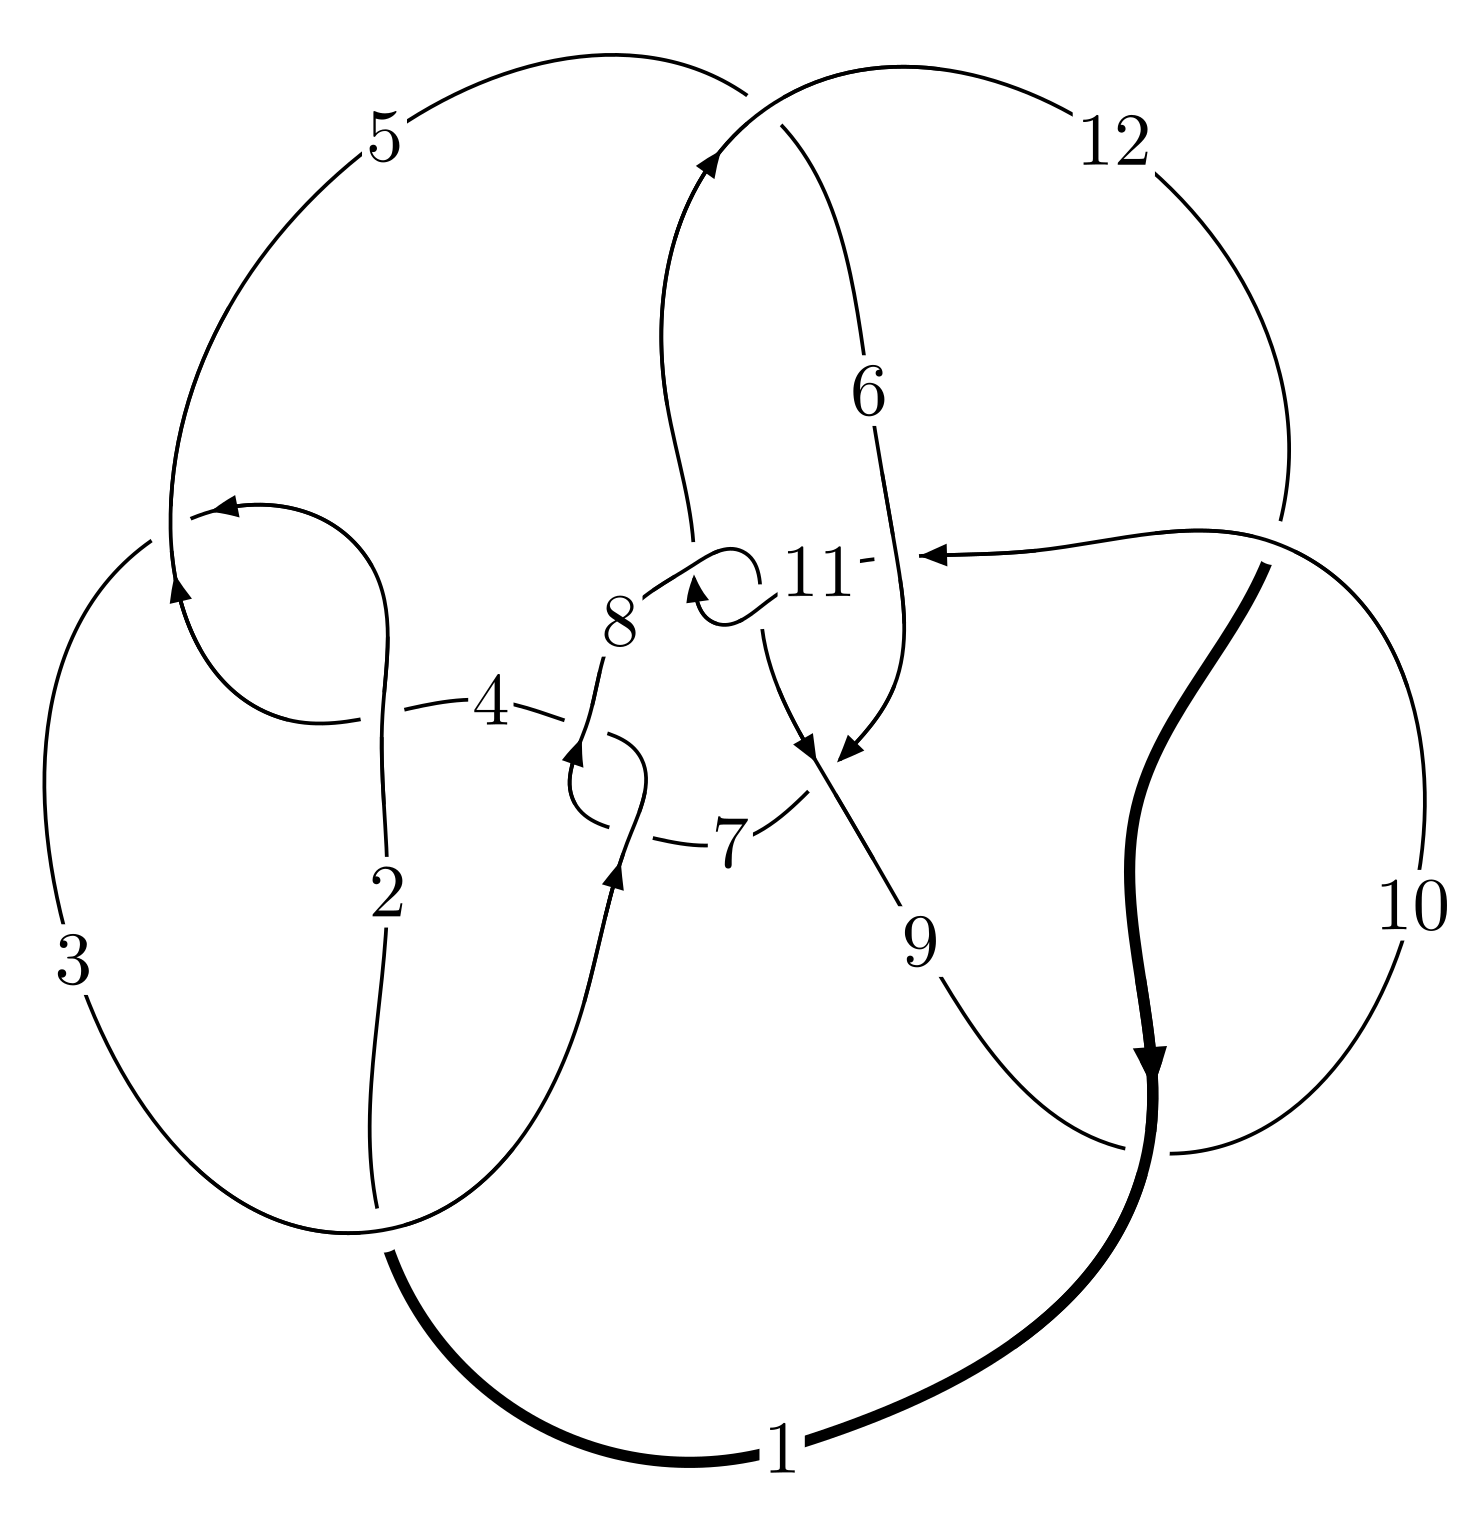
\includegraphics[width=112pt]{../../../GIT/diagram.site/Diagrams/png/2229_12n_0140.png}\\
\ \ \ A knot diagram\footnotemark}&
\allowdisplaybreaks
\textbf{Linearized knot diagam} \\
\cline{2-2}
 &
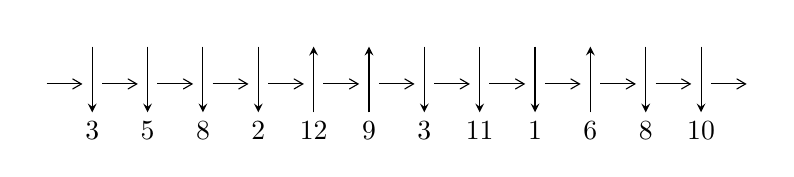
\begin{tikzpicture}[x=20pt, y=17pt]
	% nodes
	\node (C0) at (0, 0) {};
	\node (C1) at (1, 0) {};
	\node (C1U) at (1, +1) {};
	\node (C1D) at (1, -1) {3};

	\node (C2) at (2, 0) {};
	\node (C2U) at (2, +1) {};
	\node (C2D) at (2, -1) {5};

	\node (C3) at (3, 0) {};
	\node (C3U) at (3, +1) {};
	\node (C3D) at (3, -1) {8};

	\node (C4) at (4, 0) {};
	\node (C4U) at (4, +1) {};
	\node (C4D) at (4, -1) {2};

	\node (C5) at (5, 0) {};
	\node (C5U) at (5, +1) {};
	\node (C5D) at (5, -1) {12};

	\node (C6) at (6, 0) {};
	\node (C6U) at (6, +1) {};
	\node (C6D) at (6, -1) {9};

	\node (C7) at (7, 0) {};
	\node (C7U) at (7, +1) {};
	\node (C7D) at (7, -1) {3};

	\node (C8) at (8, 0) {};
	\node (C8U) at (8, +1) {};
	\node (C8D) at (8, -1) {11};

	\node (C9) at (9, 0) {};
	\node (C9U) at (9, +1) {};
	\node (C9D) at (9, -1) {1};

	\node (C10) at (10, 0) {};
	\node (C10U) at (10, +1) {};
	\node (C10D) at (10, -1) {6};

	\node (C11) at (11, 0) {};
	\node (C11U) at (11, +1) {};
	\node (C11D) at (11, -1) {8};

	\node (C12) at (12, 0) {};
	\node (C12U) at (12, +1) {};
	\node (C12D) at (12, -1) {10};
	\node (C13) at (13, 0) {};

	% arrows
	\draw[->,>={angle 60}]
	(C0) edge (C1) (C1) edge (C2) (C2) edge (C3) (C3) edge (C4) (C4) edge (C5) (C5) edge (C6) (C6) edge (C7) (C7) edge (C8) (C8) edge (C9) (C9) edge (C10) (C10) edge (C11) (C11) edge (C12) (C12) edge (C13) ;	\draw[->,>=stealth]
	(C1U) edge (C1D) (C2U) edge (C2D) (C3U) edge (C3D) (C4U) edge (C4D) (C5D) edge (C5U) (C6D) edge (C6U) (C7U) edge (C7D) (C8U) edge (C8D) (C9U) edge (C9D) (C10D) edge (C10U) (C11U) edge (C11D) (C12U) edge (C12D) ;
	\end{tikzpicture} \\
\hhline{~~} \\& 
\textbf{Solving Sequence} \\ \cline{2-2} 
 &
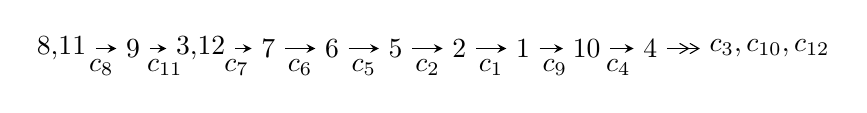
\begin{tikzpicture}[x=23pt, y=7pt]
	% node
	\node (A0) at (-1/8, 0) {8,11};
	\node (A1) at (1, 0) {9};
	\node (A2) at (33/16, 0) {3,12};
	\node (A3) at (25/8, 0) {7};
	\node (A4) at (33/8, 0) {6};
	\node (A5) at (41/8, 0) {5};
	\node (A6) at (49/8, 0) {2};
	\node (A7) at (57/8, 0) {1};
	\node (A8) at (65/8, 0) {10};
	\node (A9) at (73/8, 0) {4};
	\node (C1) at (1/2, -1) {$c_{8}$};
	\node (C2) at (3/2, -1) {$c_{11}$};
	\node (C3) at (21/8, -1) {$c_{7}$};
	\node (C4) at (29/8, -1) {$c_{6}$};
	\node (C5) at (37/8, -1) {$c_{5}$};
	\node (C6) at (45/8, -1) {$c_{2}$};
	\node (C7) at (53/8, -1) {$c_{1}$};
	\node (C8) at (61/8, -1) {$c_{9}$};
	\node (C9) at (69/8, -1) {$c_{4}$};
	\node (A10) at (11, 0) {$c_{3},c_{10},c_{12}$};

	% edge
	\draw[->,>=stealth]	
	(A0) edge (A1) (A1) edge (A2) (A2) edge (A3) (A3) edge (A4) (A4) edge (A5) (A5) edge (A6) (A6) edge (A7) (A7) edge (A8) (A8) edge (A9) ;
	\draw[->>,>={angle 60}]	
	(A9) edge (A10);
\end{tikzpicture} \\ 

\end{tabular} \\

\footnotetext{
The image of knot diagram is generated by the software ``\textbf{Draw programme}" developed by Andrew Bartholomew(\url{http://www.layer8.co.uk/maths/draw/index.htm\#Running-draw}), where we modified some parts for our purpose(\url{https://github.com/CATsTAILs/LinksPainter}).
}\phantom \\ \newline 
\centering \textbf{Ideals for irreducible components\footnotemark of $X_{\text{par}}$} 
 
\begin{align*}
I^u_{1}&=\langle 
-219034042585 u^{29}+477658347892 u^{28}+\cdots+4962190966784 b+2219335787081,\\
\phantom{I^u_{1}}&\phantom{= \langle  }-1283291111693 u^{29}+4041034486657 u^{28}+\cdots+2481095483392 a+21380565133380,\\
\phantom{I^u_{1}}&\phantom{= \langle  }u^{30}-3 u^{29}+\cdots-14 u-1\rangle \\
I^u_{2}&=\langle 
9.19271\times10^{50} u^{41}+6.53340\times10^{51} u^{40}+\cdots+1.68743\times10^{52} b+4.76895\times10^{52},\\
\phantom{I^u_{2}}&\phantom{= \langle  }-4.05666\times10^{51} u^{41}-1.46559\times10^{52} u^{40}+\cdots+1.18120\times10^{53} a-9.05537\times10^{53},\\
\phantom{I^u_{2}}&\phantom{= \langle  }u^{42}+8 u^{41}+\cdots+406 u+49\rangle \\
I^u_{3}&=\langle 
b,\;- u^3+u^2+4 a+2 u+3,\;u^4+u^2- u+1\rangle \\
I^u_{4}&=\langle 
8 a^2+b+18 a+4,\;8 a^3+20 a^2+8 a+1,\;u-1\rangle \\
I^u_{5}&=\langle 
b,\;- u^3+a- u-1,\;u^6+u^5+2 u^4+2 u^3+2 u^2+2 u+1\rangle \\
I^u_{6}&=\langle 
a u+4 b+a+u-5,\;a^2+4 a u-2 a+6 u-3,\;u^2+1\rangle \\
\\
\end{align*}
\raggedright * 6 irreducible components of $\dim_{\mathbb{C}}=0$, with total 89 representations.\\
\footnotetext{All coefficients of polynomials are rational numbers. But the coefficients are sometimes approximated in decimal forms when there is not enough margin.}
\newpage
\renewcommand{\arraystretch}{1}
\centering \section*{I. $I^u_{1}= \langle -2.19\times10^{11} u^{29}+4.78\times10^{11} u^{28}+\cdots+4.96\times10^{12} b+2.22\times10^{12},\;-1.28\times10^{12} u^{29}+4.04\times10^{12} u^{28}+\cdots+2.48\times10^{12} a+2.14\times10^{13},\;u^{30}-3 u^{29}+\cdots-14 u-1 \rangle$}
\flushleft \textbf{(i) Arc colorings}\\
\begin{tabular}{m{7pt} m{180pt} m{7pt} m{180pt} }
\flushright $a_{8}=$&$\begin{pmatrix}1\\0\end{pmatrix}$ \\
\flushright $a_{11}=$&$\begin{pmatrix}0\\u\end{pmatrix}$ \\
\flushright $a_{9}=$&$\begin{pmatrix}1\\u^2\end{pmatrix}$ \\
\flushright $a_{3}=$&$\begin{pmatrix}0.517228 u^{29}-1.62873 u^{28}+\cdots+26.8709 u-8.61739\\0.0441406 u^{29}-0.0962596 u^{28}+\cdots+1.16893 u-0.447249\end{pmatrix}$ \\
\flushright $a_{12}=$&$\begin{pmatrix}- u\\u\end{pmatrix}$ \\
\flushright $a_{7}=$&$\begin{pmatrix}0.146114 u^{29}-0.558009 u^{28}+\cdots+11.5186 u-3.67862\\0.114897 u^{29}-0.286853 u^{28}+\cdots-0.242495 u-0.299101\end{pmatrix}$ \\
\flushright $a_{6}=$&$\begin{pmatrix}0.120091 u^{29}-0.480458 u^{28}+\cdots+10.2319 u-3.49919\\0.0593413 u^{29}-0.0838619 u^{28}+\cdots-0.275735 u-0.299617\end{pmatrix}$ \\
\flushright $a_{5}=$&$\begin{pmatrix}0.120607 u^{29}-0.426449 u^{28}+\cdots+10.4168 u-3.47317\\0.0588257 u^{29}-0.137871 u^{28}+\cdots-0.460615 u-0.325639\end{pmatrix}$ \\
\flushright $a_{2}=$&$\begin{pmatrix}0.366931 u^{29}-1.21295 u^{28}+\cdots+20.1769 u-5.68931\\0.0588257 u^{29}-0.137871 u^{28}+\cdots-0.460615 u-0.325639\end{pmatrix}$ \\
\flushright $a_{1}=$&$\begin{pmatrix}-0.0625000 u^{29}+0.125000 u^{28}+\cdots+2.93750 u+0.0625000\\\frac{1}{16} u^{29}-\frac{1}{8} u^{28}+\cdots-\frac{31}{16} u-\frac{1}{16}\end{pmatrix}$ \\
\flushright $a_{10}=$&$\begin{pmatrix}\frac{1}{16} u^{29}-\frac{1}{4} u^{28}+\cdots+\frac{13}{16} u+\frac{17}{16}\\-0.0625000 u^{29}+0.250000 u^{28}+\cdots-0.812500 u-0.0625000\end{pmatrix}$ \\
\flushright $a_{4}=$&$\begin{pmatrix}0.473087 u^{29}-1.53247 u^{28}+\cdots+25.7020 u-8.17014\\0.0441406 u^{29}-0.0962596 u^{28}+\cdots+1.16893 u-0.447249\end{pmatrix}$\\&\end{tabular}
\flushleft \textbf{(ii) Obstruction class $= -1$}\\~\\
\flushleft \textbf{(iii) Cusp Shapes $= -\frac{29246499640993}{39697527734272} u^{29}+\frac{4877178426605}{2481095483392} u^{28}+\cdots-\frac{648015885883539}{39697527734272} u-\frac{374986321947515}{39697527734272}$}\\~\\
\newpage\renewcommand{\arraystretch}{1}
\flushleft \textbf{(iv) u-Polynomials at the component}\newline \\
\begin{tabular}{m{50pt}|m{274pt}}
Crossings & \hspace{64pt}u-Polynomials at each crossing \\
\hline $$\begin{aligned}c_{1}\end{aligned}$$&$\begin{aligned}
&u^{30}+14 u^{29}+\cdots-2399 u+256
\end{aligned}$\\
\hline $$\begin{aligned}c_{2},c_{4}\end{aligned}$$&$\begin{aligned}
&u^{30}-6 u^{29}+\cdots-31 u+16
\end{aligned}$\\
\hline $$\begin{aligned}c_{3},c_{7}\end{aligned}$$&$\begin{aligned}
&u^{30}-2 u^{29}+\cdots-96 u-256
\end{aligned}$\\
\hline $$\begin{aligned}c_{5},c_{6}\end{aligned}$$&$\begin{aligned}
&8(8 u^{30}+20 u^{29}+\cdots+12 u+4)
\end{aligned}$\\
\hline $$\begin{aligned}c_{8},c_{9},c_{11}\\c_{12}\end{aligned}$$&$\begin{aligned}
&u^{30}+3 u^{29}+\cdots+14 u-1
\end{aligned}$\\
\hline $$\begin{aligned}c_{10}\end{aligned}$$&$\begin{aligned}
&u^{30}-6 u^{29}+\cdots+64 u+256
\end{aligned}$\\
\hline
\end{tabular}\\~\\
\newpage\renewcommand{\arraystretch}{1}
\flushleft \textbf{(v) Riley Polynomials at the component}\newline \\
\begin{tabular}{m{50pt}|m{274pt}}
Crossings & \hspace{64pt}Riley Polynomials at each crossing \\
\hline $$\begin{aligned}c_{1}\end{aligned}$$&$\begin{aligned}
&y^{30}+10 y^{29}+\cdots-6849345 y+65536
\end{aligned}$\\
\hline $$\begin{aligned}c_{2},c_{4}\end{aligned}$$&$\begin{aligned}
&y^{30}-14 y^{29}+\cdots+2399 y+256
\end{aligned}$\\
\hline $$\begin{aligned}c_{3},c_{7}\end{aligned}$$&$\begin{aligned}
&y^{30}+18 y^{29}+\cdots+76800 y+65536
\end{aligned}$\\
\hline $$\begin{aligned}c_{5},c_{6}\end{aligned}$$&$\begin{aligned}
&64(64 y^{30}-1360 y^{29}+\cdots-192 y+16)
\end{aligned}$\\
\hline $$\begin{aligned}c_{8},c_{9},c_{11}\\c_{12}\end{aligned}$$&$\begin{aligned}
&y^{30}+23 y^{29}+\cdots-290 y+1
\end{aligned}$\\
\hline $$\begin{aligned}c_{10}\end{aligned}$$&$\begin{aligned}
&y^{30}+6 y^{29}+\cdots-1789952 y+65536
\end{aligned}$\\
\hline
\end{tabular}\\~\\
\newpage\flushleft \textbf{(vi) Complex Volumes and Cusp Shapes}
$$\begin{array}{c|c|c}  
\text{Solutions to }I^u_{1}& \I (\text{vol} + \sqrt{-1}CS) & \text{Cusp shape}\\
 \hline 
\begin{aligned}
u &= \phantom{-}0.151717 + 0.986186 I \\
a &= -1.190140 - 0.027428 I \\
b &= \phantom{-}1.54321 - 0.20318 I\end{aligned}
 & -5.68347 - 0.58233 I & -8.3451 + 12.8590 I \\ \hline\begin{aligned}
u &= \phantom{-}0.151717 - 0.986186 I \\
a &= -1.190140 + 0.027428 I \\
b &= \phantom{-}1.54321 + 0.20318 I\end{aligned}
 & -5.68347 + 0.58233 I & -8.3451 - 12.8590 I \\ \hline\begin{aligned}
u &= \phantom{-}0.783732 + 0.743673 I \\
a &= \phantom{-}0.631228 - 0.256038 I \\
b &= -0.083764 + 0.794094 I\end{aligned}
 & -1.33282 - 2.23553 I & -4.59779 + 3.41546 I \\ \hline\begin{aligned}
u &= \phantom{-}0.783732 - 0.743673 I \\
a &= \phantom{-}0.631228 + 0.256038 I \\
b &= -0.083764 - 0.794094 I\end{aligned}
 & -1.33282 + 2.23553 I & -4.59779 - 3.41546 I \\ \hline\begin{aligned}
u &= \phantom{-}1.09098\phantom{ +0.000000I} \\
a &= \phantom{-}1.70930\phantom{ +0.000000I} \\
b &= \phantom{-}0.608605\phantom{ +0.000000I}\end{aligned}
 & -2.65754\phantom{ +0.000000I} & \phantom{-}30.3480\phantom{ +0.000000I} \\ \hline\begin{aligned}
u &= -0.576049 + 1.073970 I \\
a &= -0.261951 - 0.195372 I \\
b &= -0.151381 + 0.594028 I\end{aligned}
 & \phantom{-}1.34016 + 8.01200 I & \phantom{-}2.34579 - 12.49324 I \\ \hline\begin{aligned}
u &= -0.576049 - 1.073970 I \\
a &= -0.261951 + 0.195372 I \\
b &= -0.151381 - 0.594028 I\end{aligned}
 & \phantom{-}1.34016 - 8.01200 I & \phantom{-}2.34579 + 12.49324 I \\ \hline\begin{aligned}
u &= \phantom{-}0.625133 + 0.199278 I \\
a &= \phantom{-}1.38297 + 2.15219 I \\
b &= \phantom{-}0.386290 - 0.372621 I\end{aligned}
 & -2.83148 - 0.66530 I & -18.2240 - 6.7846 I \\ \hline\begin{aligned}
u &= \phantom{-}0.625133 - 0.199278 I \\
a &= \phantom{-}1.38297 - 2.15219 I \\
b &= \phantom{-}0.386290 + 0.372621 I\end{aligned}
 & -2.83148 + 0.66530 I & -18.2240 + 6.7846 I \\ \hline\begin{aligned}
u &= -0.117957 + 1.367060 I \\
a &= \phantom{-}0.699932 - 0.475481 I \\
b &= -1.78516 + 0.43773 I\end{aligned}
 & \phantom{-}6.76007 + 1.66777 I & \phantom{-}0.57274 - 1.46728 I\\
 \hline 
 \end{array}$$\newpage$$\begin{array}{c|c|c}  
\text{Solutions to }I^u_{1}& \I (\text{vol} + \sqrt{-1}CS) & \text{Cusp shape}\\
 \hline 
\begin{aligned}
u &= -0.117957 - 1.367060 I \\
a &= \phantom{-}0.699932 + 0.475481 I \\
b &= -1.78516 - 0.43773 I\end{aligned}
 & \phantom{-}6.76007 - 1.66777 I & \phantom{-}0.57274 + 1.46728 I \\ \hline\begin{aligned}
u &= -0.244597 + 1.352860 I \\
a &= \phantom{-}0.31073 + 1.77800 I \\
b &= -0.22783 - 1.65229 I\end{aligned}
 & \phantom{-}5.09939 + 5.42433 I & -0.68852 - 4.20178 I \\ \hline\begin{aligned}
u &= -0.244597 - 1.352860 I \\
a &= \phantom{-}0.31073 - 1.77800 I \\
b &= -0.22783 + 1.65229 I\end{aligned}
 & \phantom{-}5.09939 - 5.42433 I & -0.68852 + 4.20178 I \\ \hline\begin{aligned}
u &= \phantom{-}0.259417 + 1.365310 I \\
a &= -0.19856 + 1.74019 I \\
b &= -0.91810 - 1.71117 I\end{aligned}
 & \phantom{-}10.78970 - 8.07891 I & -0.53452 + 5.22614 I \\ \hline\begin{aligned}
u &= \phantom{-}0.259417 - 1.365310 I \\
a &= -0.19856 - 1.74019 I \\
b &= -0.91810 + 1.71117 I\end{aligned}
 & \phantom{-}10.78970 + 8.07891 I & -0.53452 - 5.22614 I \\ \hline\begin{aligned}
u &= -0.35445 + 1.40429 I \\
a &= -0.544865 + 0.390463 I \\
b &= \phantom{-}1.65162 + 0.07394 I\end{aligned}
 & \phantom{-}7.38806 + 8.84406 I & -1.28461 - 6.03116 I \\ \hline\begin{aligned}
u &= -0.35445 - 1.40429 I \\
a &= -0.544865 - 0.390463 I \\
b &= \phantom{-}1.65162 - 0.07394 I\end{aligned}
 & \phantom{-}7.38806 - 8.84406 I & -1.28461 + 6.03116 I \\ \hline\begin{aligned}
u &= \phantom{-}0.06550 + 1.45294 I \\
a &= -0.04154 - 1.68423 I \\
b &= \phantom{-}0.69837 + 1.94525 I\end{aligned}
 & \phantom{-}13.33180 - 0.21203 I & \phantom{-}1.73134 + 0. I\phantom{ +0.000000I} \\ \hline\begin{aligned}
u &= \phantom{-}0.06550 - 1.45294 I \\
a &= -0.04154 + 1.68423 I \\
b &= \phantom{-}0.69837 - 1.94525 I\end{aligned}
 & \phantom{-}13.33180 + 0.21203 I & \phantom{-}1.73134 + 0. I\phantom{ +0.000000I} \\ \hline\begin{aligned}
u &= \phantom{-}0.339570 + 0.379677 I \\
a &= \phantom{-}0.592119 + 0.913683 I \\
b &= -0.452974 - 0.318485 I\end{aligned}
 & -0.505428 - 1.105530 I & -5.83661 + 6.57696 I\\
 \hline 
 \end{array}$$\newpage$$\begin{array}{c|c|c}  
\text{Solutions to }I^u_{1}& \I (\text{vol} + \sqrt{-1}CS) & \text{Cusp shape}\\
 \hline 
\begin{aligned}
u &= \phantom{-}0.339570 - 0.379677 I \\
a &= \phantom{-}0.592119 - 0.913683 I \\
b &= -0.452974 + 0.318485 I\end{aligned}
 & -0.505428 + 1.105530 I & -5.83661 - 6.57696 I \\ \hline\begin{aligned}
u &= \phantom{-}1.52530 + 0.11249 I \\
a &= \phantom{-}0.155403 + 0.304847 I \\
b &= \phantom{-}0.24118 - 1.48607 I\end{aligned}
 & \phantom{-}2.40331 + 3.17859 I & \phantom{-0.000000 } 0. - 3.79440 I \\ \hline\begin{aligned}
u &= \phantom{-}1.52530 - 0.11249 I \\
a &= \phantom{-}0.155403 - 0.304847 I \\
b &= \phantom{-}0.24118 + 1.48607 I\end{aligned}
 & \phantom{-}2.40331 - 3.17859 I & \phantom{-0.000000 -}0. + 3.79440 I \\ \hline\begin{aligned}
u &= -0.58141 + 1.45298 I \\
a &= \phantom{-}0.76540 + 1.55713 I \\
b &= \phantom{-}0.78764 - 1.58037 I\end{aligned}
 & \phantom{-}12.0126 + 17.2447 I & -2.29441 - 8.43337 I \\ \hline\begin{aligned}
u &= -0.58141 - 1.45298 I \\
a &= \phantom{-}0.76540 - 1.55713 I \\
b &= \phantom{-}0.78764 + 1.58037 I\end{aligned}
 & \phantom{-}12.0126 - 17.2447 I & -2.29441 + 8.43337 I \\ \hline\begin{aligned}
u &= -0.414284 + 0.113025 I \\
a &= \phantom{-}0.170265 - 1.051000 I \\
b &= -0.229191 - 1.205720 I\end{aligned}
 & \phantom{-}2.31731 - 2.61856 I & \phantom{-}1.56244 + 2.01080 I \\ \hline\begin{aligned}
u &= -0.414284 - 0.113025 I \\
a &= \phantom{-}0.170265 + 1.051000 I \\
b &= -0.229191 + 1.205720 I\end{aligned}
 & \phantom{-}2.31731 + 2.61856 I & \phantom{-}1.56244 - 2.01080 I \\ \hline\begin{aligned}
u &= -0.47748 + 1.50384 I \\
a &= -0.58934 - 1.58578 I \\
b &= -0.50245 + 1.81791 I\end{aligned}
 & \phantom{-}14.1647 + 9.9224 I & \phantom{-0.000000 } 0. - 4.39684 I \\ \hline\begin{aligned}
u &= -0.47748 - 1.50384 I \\
a &= -0.58934 + 1.58578 I \\
b &= -0.50245 - 1.81791 I\end{aligned}
 & \phantom{-}14.1647 - 9.9224 I & \phantom{-0.000000 -}0. + 4.39684 I \\ \hline\begin{aligned}
u &= -0.0592723\phantom{ +0.000000I} \\
a &= -10.2226\phantom{ +0.000000I} \\
b &= -0.523532\phantom{ +0.000000I}\end{aligned}
 & -1.19030\phantom{ +0.000000I} & -8.24210\phantom{ +0.000000I}\\
 \hline 
 \end{array}$$\newpage\newpage\renewcommand{\arraystretch}{1}
\centering \section*{II. $I^u_{2}= \langle 9.19\times10^{50} u^{41}+6.53\times10^{51} u^{40}+\cdots+1.69\times10^{52} b+4.77\times10^{52},\;-4.06\times10^{51} u^{41}-1.47\times10^{52} u^{40}+\cdots+1.18\times10^{53} a-9.06\times10^{53},\;u^{42}+8 u^{41}+\cdots+406 u+49 \rangle$}
\flushleft \textbf{(i) Arc colorings}\\
\begin{tabular}{m{7pt} m{180pt} m{7pt} m{180pt} }
\flushright $a_{8}=$&$\begin{pmatrix}1\\0\end{pmatrix}$ \\
\flushright $a_{11}=$&$\begin{pmatrix}0\\u\end{pmatrix}$ \\
\flushright $a_{9}=$&$\begin{pmatrix}1\\u^2\end{pmatrix}$ \\
\flushright $a_{3}=$&$\begin{pmatrix}0.0343435 u^{41}+0.124076 u^{40}+\cdots+50.6244 u+7.66624\\-0.0544776 u^{41}-0.387181 u^{40}+\cdots-17.0063 u-2.82616\end{pmatrix}$ \\
\flushright $a_{12}=$&$\begin{pmatrix}- u\\u\end{pmatrix}$ \\
\flushright $a_{7}=$&$\begin{pmatrix}-0.137949 u^{41}-1.03303 u^{40}+\cdots-26.6535 u-2.02469\\-0.0157309 u^{41}-0.0881611 u^{40}+\cdots+22.8491 u+3.77512\end{pmatrix}$ \\
\flushright $a_{6}=$&$\begin{pmatrix}-0.162962 u^{41}-1.21826 u^{40}+\cdots-71.3909 u-9.25731\\-0.0118963 u^{41}-0.0998927 u^{40}+\cdots+18.0364 u+3.04637\end{pmatrix}$ \\
\flushright $a_{5}=$&$\begin{pmatrix}-0.146119 u^{41}-1.10192 u^{40}+\cdots-47.1902 u-5.30246\\-0.0287391 u^{41}-0.216234 u^{40}+\cdots-6.16428 u-0.908484\end{pmatrix}$ \\
\flushright $a_{2}=$&$\begin{pmatrix}0.187628 u^{41}+1.31124 u^{40}+\cdots+100.721 u+14.2062\\-0.0287391 u^{41}-0.216234 u^{40}+\cdots-6.16428 u-0.908484\end{pmatrix}$ \\
\flushright $a_{1}=$&$\begin{pmatrix}0.0204082 u^{41}+0.163265 u^{40}+\cdots+36.6122 u+8.28571\\0.0941921 u^{41}+0.708146 u^{40}+\cdots+54.1974 u+8.58973\end{pmatrix}$ \\
\flushright $a_{10}=$&$\begin{pmatrix}0.175301 u^{41}+1.30821 u^{40}+\cdots+114.966 u+16.9746\\-1\end{pmatrix}$ \\
\flushright $a_{4}=$&$\begin{pmatrix}0.0888211 u^{41}+0.511257 u^{40}+\cdots+67.6307 u+10.4924\\-0.0544776 u^{41}-0.387181 u^{40}+\cdots-17.0063 u-2.82616\end{pmatrix}$\\&\end{tabular}
\flushleft \textbf{(ii) Obstruction class $= -1$}\\~\\
\flushleft \textbf{(iii) Cusp Shapes $= -0.137513 u^{41}-1.10677 u^{40}+\cdots-86.1411 u-17.7083$}\\~\\
\newpage\renewcommand{\arraystretch}{1}
\flushleft \textbf{(iv) u-Polynomials at the component}\newline \\
\begin{tabular}{m{50pt}|m{274pt}}
Crossings & \hspace{64pt}u-Polynomials at each crossing \\
\hline $$\begin{aligned}c_{1}\end{aligned}$$&$\begin{aligned}
&(u^{21}+6 u^{20}+\cdots-2 u+1)^{2}
\end{aligned}$\\
\hline $$\begin{aligned}c_{2},c_{4}\end{aligned}$$&$\begin{aligned}
&(u^{21}-4 u^{20}+\cdots-2 u+1)^{2}
\end{aligned}$\\
\hline $$\begin{aligned}c_{3},c_{7}\end{aligned}$$&$\begin{aligned}
&(u^{21}- u^{20}+\cdots+4 u+8)^{2}
\end{aligned}$\\
\hline $$\begin{aligned}c_{5},c_{6}\end{aligned}$$&$\begin{aligned}
&u^{42}+8 u^{41}+\cdots+859266 u+387139
\end{aligned}$\\
\hline $$\begin{aligned}c_{8},c_{9},c_{11}\\c_{12}\end{aligned}$$&$\begin{aligned}
&u^{42}-8 u^{41}+\cdots-406 u+49
\end{aligned}$\\
\hline $$\begin{aligned}c_{10}\end{aligned}$$&$\begin{aligned}
&(u^{21}+2 u^{20}+\cdots+u-1)^{2}
\end{aligned}$\\
\hline
\end{tabular}\\~\\
\newpage\renewcommand{\arraystretch}{1}
\flushleft \textbf{(v) Riley Polynomials at the component}\newline \\
\begin{tabular}{m{50pt}|m{274pt}}
Crossings & \hspace{64pt}Riley Polynomials at each crossing \\
\hline $$\begin{aligned}c_{1}\end{aligned}$$&$\begin{aligned}
&(y^{21}+22 y^{20}+\cdots+66 y-1)^{2}
\end{aligned}$\\
\hline $$\begin{aligned}c_{2},c_{4}\end{aligned}$$&$\begin{aligned}
&(y^{21}-6 y^{20}+\cdots-2 y-1)^{2}
\end{aligned}$\\
\hline $$\begin{aligned}c_{3},c_{7}\end{aligned}$$&$\begin{aligned}
&(y^{21}+21 y^{20}+\cdots-176 y-64)^{2}
\end{aligned}$\\
\hline $$\begin{aligned}c_{5},c_{6}\end{aligned}$$&$\begin{aligned}
&y^{42}-26 y^{41}+\cdots-934716639340 y+149876605321
\end{aligned}$\\
\hline $$\begin{aligned}c_{8},c_{9},c_{11}\\c_{12}\end{aligned}$$&$\begin{aligned}
&y^{42}+30 y^{41}+\cdots+10976 y+2401
\end{aligned}$\\
\hline $$\begin{aligned}c_{10}\end{aligned}$$&$\begin{aligned}
&(y^{21}-8 y^{20}+\cdots+17 y-1)^{2}
\end{aligned}$\\
\hline
\end{tabular}\\~\\
\newpage\flushleft \textbf{(vi) Complex Volumes and Cusp Shapes}
$$\begin{array}{c|c|c}  
\text{Solutions to }I^u_{2}& \I (\text{vol} + \sqrt{-1}CS) & \text{Cusp shape}\\
 \hline 
\begin{aligned}
u &= -0.041887 + 1.002630 I \\
a &= -8.74756 - 5.85633 I \\
b &= -0.492750\phantom{ +0.000000I}\end{aligned}
 & \phantom{-}2.07989\phantom{ +0.000000I} & -13.37190 + 0. I\phantom{ +0.000000I} \\ \hline\begin{aligned}
u &= -0.041887 - 1.002630 I \\
a &= -8.74756 + 5.85633 I \\
b &= -0.492750\phantom{ +0.000000I}\end{aligned}
 & \phantom{-}2.07989\phantom{ +0.000000I} & -13.37190 + 0. I\phantom{ +0.000000I} \\ \hline\begin{aligned}
u &= -0.870370 + 0.220126 I \\
a &= \phantom{-}1.199530 - 0.425810 I \\
b &= \phantom{-}1.088250 - 0.021385 I\end{aligned}
 & \phantom{-}2.22124 + 4.45806 I & -4.43689 - 6.14529 I \\ \hline\begin{aligned}
u &= -0.870370 - 0.220126 I \\
a &= \phantom{-}1.199530 + 0.425810 I \\
b &= \phantom{-}1.088250 + 0.021385 I\end{aligned}
 & \phantom{-}2.22124 - 4.45806 I & -4.43689 + 6.14529 I \\ \hline\begin{aligned}
u &= -0.769906 + 0.433901 I \\
a &= \phantom{-}0.483221 - 0.092871 I \\
b &= -0.006772 - 0.621655 I\end{aligned}
 & -0.56968 - 2.93752 I & -1.02400 + 3.43881 I \\ \hline\begin{aligned}
u &= -0.769906 - 0.433901 I \\
a &= \phantom{-}0.483221 + 0.092871 I \\
b &= -0.006772 + 0.621655 I\end{aligned}
 & -0.56968 + 2.93752 I & -1.02400 - 3.43881 I \\ \hline\begin{aligned}
u &= \phantom{-}0.600601 + 0.944887 I \\
a &= -0.154802 + 0.082043 I \\
b &= -0.006772 - 0.621655 I\end{aligned}
 & -0.56968 - 2.93752 I & \phantom{-0.000000 -}0. + 3.43881 I \\ \hline\begin{aligned}
u &= \phantom{-}0.600601 - 0.944887 I \\
a &= -0.154802 - 0.082043 I \\
b &= -0.006772 + 0.621655 I\end{aligned}
 & -0.56968 + 2.93752 I & \phantom{-0.000000 } 0. - 3.43881 I \\ \hline\begin{aligned}
u &= -0.475850 + 1.016220 I \\
a &= \phantom{-}0.272799 + 0.705259 I \\
b &= \phantom{-}0.528856 + 0.467306 I\end{aligned}
 & \phantom{-}4.75904 + 0.34630 I & \phantom{-}1.96536 + 0. I\phantom{ +0.000000I} \\ \hline\begin{aligned}
u &= -0.475850 - 1.016220 I \\
a &= \phantom{-}0.272799 - 0.705259 I \\
b &= \phantom{-}0.528856 - 0.467306 I\end{aligned}
 & \phantom{-}4.75904 - 0.34630 I & \phantom{-}1.96536 + 0. I\phantom{ +0.000000I}\\
 \hline 
 \end{array}$$\newpage$$\begin{array}{c|c|c}  
\text{Solutions to }I^u_{2}& \I (\text{vol} + \sqrt{-1}CS) & \text{Cusp shape}\\
 \hline 
\begin{aligned}
u &= \phantom{-}0.053090 + 1.155400 I \\
a &= -0.058655 - 0.325592 I \\
b &= -0.899194 - 0.226112 I\end{aligned}
 & \phantom{-}1.45515 - 0.21101 I & -6.00000 + 0. I\phantom{ +0.000000I} \\ \hline\begin{aligned}
u &= \phantom{-}0.053090 - 1.155400 I \\
a &= -0.058655 + 0.325592 I \\
b &= -0.899194 + 0.226112 I\end{aligned}
 & \phantom{-}1.45515 + 0.21101 I & -6.00000 + 0. I\phantom{ +0.000000I} \\ \hline\begin{aligned}
u &= \phantom{-}0.216321 + 1.202960 I \\
a &= -0.33507 - 2.15389 I \\
b &= -0.157544 + 0.891019 I\end{aligned}
 & \phantom{-}0.26332 - 2.36605 I & \phantom{-0.000000 } 0 \\ \hline\begin{aligned}
u &= \phantom{-}0.216321 - 1.202960 I \\
a &= -0.33507 + 2.15389 I \\
b &= -0.157544 - 0.891019 I\end{aligned}
 & \phantom{-}0.26332 + 2.36605 I & \phantom{-0.000000 } 0 \\ \hline\begin{aligned}
u &= \phantom{-}0.474335 + 0.591031 I \\
a &= \phantom{-}1.05367 + 1.22545 I \\
b &= \phantom{-}0.00145 + 1.46011 I\end{aligned}
 & \phantom{-}6.58039 + 1.36266 I & -4.18856 - 2.27516 I \\ \hline\begin{aligned}
u &= \phantom{-}0.474335 - 0.591031 I \\
a &= \phantom{-}1.05367 - 1.22545 I \\
b &= \phantom{-}0.00145 - 1.46011 I\end{aligned}
 & \phantom{-}6.58039 - 1.36266 I & -4.18856 + 2.27516 I \\ \hline\begin{aligned}
u &= -0.185639 + 1.238440 I \\
a &= -0.70977 - 2.01041 I \\
b &= -0.45321 + 1.45865 I\end{aligned}
 & \phantom{-}5.71484 + 4.94435 I & \phantom{-0.000000 } 0 \\ \hline\begin{aligned}
u &= -0.185639 - 1.238440 I \\
a &= -0.70977 + 2.01041 I \\
b &= -0.45321 - 1.45865 I\end{aligned}
 & \phantom{-}5.71484 - 4.94435 I & \phantom{-0.000000 } 0 \\ \hline\begin{aligned}
u &= -0.021801 + 1.271800 I \\
a &= \phantom{-}0.50394 + 2.30405 I \\
b &= \phantom{-}0.00145 - 1.46011 I\end{aligned}
 & \phantom{-}6.58039 - 1.36266 I & \phantom{-0.000000 } 0 \\ \hline\begin{aligned}
u &= -0.021801 - 1.271800 I \\
a &= \phantom{-}0.50394 - 2.30405 I \\
b &= \phantom{-}0.00145 + 1.46011 I\end{aligned}
 & \phantom{-}6.58039 + 1.36266 I & \phantom{-0.000000 } 0\\
 \hline 
 \end{array}$$\newpage$$\begin{array}{c|c|c}  
\text{Solutions to }I^u_{2}& \I (\text{vol} + \sqrt{-1}CS) & \text{Cusp shape}\\
 \hline 
\begin{aligned}
u &= -1.252620 + 0.261440 I \\
a &= -0.093957 - 0.166544 I \\
b &= -0.15224 + 1.62071 I\end{aligned}
 & \phantom{-}8.50490 + 3.89686 I & \phantom{-0.000000 } 0 \\ \hline\begin{aligned}
u &= -1.252620 - 0.261440 I \\
a &= -0.093957 + 0.166544 I \\
b &= -0.15224 - 1.62071 I\end{aligned}
 & \phantom{-}8.50490 - 3.89686 I & \phantom{-0.000000 } 0 \\ \hline\begin{aligned}
u &= -1.302650 + 0.047271 I \\
a &= \phantom{-}0.370885 + 0.223986 I \\
b &= \phantom{-}0.55439 - 1.54207 I\end{aligned}
 & \phantom{-}7.25306 + 10.68720 I & \phantom{-0.000000 } 0 \\ \hline\begin{aligned}
u &= -1.302650 - 0.047271 I \\
a &= \phantom{-}0.370885 - 0.223986 I \\
b &= \phantom{-}0.55439 + 1.54207 I\end{aligned}
 & \phantom{-}7.25306 - 10.68720 I & \phantom{-0.000000 } 0 \\ \hline\begin{aligned}
u &= -0.226174 + 1.289570 I \\
a &= \phantom{-}0.560692 + 0.745306 I \\
b &= \phantom{-}0.528856 - 0.467306 I\end{aligned}
 & \phantom{-}4.75904 - 0.34630 I & \phantom{-0.000000 } 0 \\ \hline\begin{aligned}
u &= -0.226174 - 1.289570 I \\
a &= \phantom{-}0.560692 - 0.745306 I \\
b &= \phantom{-}0.528856 + 0.467306 I\end{aligned}
 & \phantom{-}4.75904 + 0.34630 I & \phantom{-0.000000 } 0 \\ \hline\begin{aligned}
u &= \phantom{-}0.588336 + 0.271246 I \\
a &= -0.350608 - 1.017080 I \\
b &= -0.45321 - 1.45865 I\end{aligned}
 & \phantom{-}5.71484 - 4.94435 I & -5.24866 + 2.70559 I \\ \hline\begin{aligned}
u &= \phantom{-}0.588336 - 0.271246 I \\
a &= -0.350608 + 1.017080 I \\
b &= -0.45321 + 1.45865 I\end{aligned}
 & \phantom{-}5.71484 + 4.94435 I & -5.24866 - 2.70559 I \\ \hline\begin{aligned}
u &= \phantom{-}0.319588 + 1.353120 I \\
a &= -0.014969 - 0.198168 I \\
b &= \phantom{-}1.088250 + 0.021385 I\end{aligned}
 & \phantom{-}2.22124 - 4.45806 I & \phantom{-0.000000 } 0 \\ \hline\begin{aligned}
u &= \phantom{-}0.319588 - 1.353120 I \\
a &= -0.014969 + 0.198168 I \\
b &= \phantom{-}1.088250 - 0.021385 I\end{aligned}
 & \phantom{-}2.22124 + 4.45806 I & \phantom{-0.000000 } 0\\
 \hline 
 \end{array}$$\newpage$$\begin{array}{c|c|c}  
\text{Solutions to }I^u_{2}& \I (\text{vol} + \sqrt{-1}CS) & \text{Cusp shape}\\
 \hline 
\begin{aligned}
u &= -0.579219 + 0.187158 I \\
a &= -1.56373 + 0.83045 I \\
b &= -0.157544 - 0.891019 I\end{aligned}
 & \phantom{-}0.26332 + 2.36605 I & -4.59037 - 2.67274 I \\ \hline\begin{aligned}
u &= -0.579219 - 0.187158 I \\
a &= -1.56373 - 0.83045 I \\
b &= -0.157544 + 0.891019 I\end{aligned}
 & \phantom{-}0.26332 - 2.36605 I & -4.59037 + 2.67274 I \\ \hline\begin{aligned}
u &= -0.239978 + 0.362151 I \\
a &= -3.20155 + 1.86451 I \\
b &= -0.899194 + 0.226112 I\end{aligned}
 & \phantom{-}1.45515 + 0.21101 I & -7.18710 - 0.57244 I \\ \hline\begin{aligned}
u &= -0.239978 - 0.362151 I \\
a &= -3.20155 - 1.86451 I \\
b &= -0.899194 - 0.226112 I\end{aligned}
 & \phantom{-}1.45515 - 0.21101 I & -7.18710 + 0.57244 I \\ \hline\begin{aligned}
u &= \phantom{-}0.62069 + 1.53093 I \\
a &= \phantom{-}0.66906 - 1.34449 I \\
b &= \phantom{-}0.55439 + 1.54207 I\end{aligned}
 & \phantom{-}7.25306 - 10.68720 I & \phantom{-0.000000 } 0 \\ \hline\begin{aligned}
u &= \phantom{-}0.62069 - 1.53093 I \\
a &= \phantom{-}0.66906 + 1.34449 I \\
b &= \phantom{-}0.55439 - 1.54207 I\end{aligned}
 & \phantom{-}7.25306 + 10.68720 I & \phantom{-0.000000 } 0 \\ \hline\begin{aligned}
u &= \phantom{-}0.45894 + 1.59821 I \\
a &= -0.42722 + 1.36484 I \\
b &= -0.15224 - 1.62071 I\end{aligned}
 & \phantom{-}8.50490 - 3.89686 I & \phantom{-0.000000 } 0 \\ \hline\begin{aligned}
u &= \phantom{-}0.45894 - 1.59821 I \\
a &= -0.42722 - 1.36484 I \\
b &= -0.15224 + 1.62071 I\end{aligned}
 & \phantom{-}8.50490 + 3.89686 I & \phantom{-0.000000 } 0 \\ \hline\begin{aligned}
u &= -0.76320 + 1.48676 I \\
a &= \phantom{-}0.794802 + 1.042100 I \\
b &= \phantom{-}0.24239 - 1.67299 I\end{aligned}
 & \phantom{-}12.12580 + 3.51416 I & \phantom{-0.000000 } 0 \\ \hline\begin{aligned}
u &= -0.76320 - 1.48676 I \\
a &= \phantom{-}0.794802 - 1.042100 I \\
b &= \phantom{-}0.24239 + 1.67299 I\end{aligned}
 & \phantom{-}12.12580 - 3.51416 I & \phantom{-0.000000 } 0\\
 \hline 
 \end{array}$$\newpage$$\begin{array}{c|c|c}  
\text{Solutions to }I^u_{2}& \I (\text{vol} + \sqrt{-1}CS) & \text{Cusp shape}\\
 \hline 
\begin{aligned}
u &= -0.60260 + 1.60806 I \\
a &= -0.536403 - 1.053510 I \\
b &= \phantom{-}0.24239 + 1.67299 I\end{aligned}
 & \phantom{-}12.12580 - 3.51416 I & \phantom{-0.000000 } 0 \\ \hline\begin{aligned}
u &= -0.60260 - 1.60806 I \\
a &= -0.536403 + 1.053510 I \\
b &= \phantom{-}0.24239 - 1.67299 I\end{aligned}
 & \phantom{-}12.12580 + 3.51416 I & \phantom{-0.000000 } 0\\
 \hline 
 \end{array}$$\newpage\newpage\renewcommand{\arraystretch}{1}
\centering \section*{III. $I^u_{3}= \langle b,\;- u^3+u^2+4 a+2 u+3,\;u^4+u^2- u+1 \rangle$}
\flushleft \textbf{(i) Arc colorings}\\
\begin{tabular}{m{7pt} m{180pt} m{7pt} m{180pt} }
\flushright $a_{8}=$&$\begin{pmatrix}1\\0\end{pmatrix}$ \\
\flushright $a_{11}=$&$\begin{pmatrix}0\\u\end{pmatrix}$ \\
\flushright $a_{9}=$&$\begin{pmatrix}1\\u^2\end{pmatrix}$ \\
\flushright $a_{3}=$&$\begin{pmatrix}\frac{1}{4} u^3-\frac{1}{4} u^2-\frac{1}{2} u-\frac{3}{4}\\0\end{pmatrix}$ \\
\flushright $a_{12}=$&$\begin{pmatrix}- u\\u\end{pmatrix}$ \\
\flushright $a_{7}=$&$\begin{pmatrix}1\\0\end{pmatrix}$ \\
\flushright $a_{6}=$&$\begin{pmatrix}u^2+1\\- u^2+u-1\end{pmatrix}$ \\
\flushright $a_{5}=$&$\begin{pmatrix}- u^3+u^2+1\\u^3- u^2+u-1\end{pmatrix}$ \\
\flushright $a_{2}=$&$\begin{pmatrix}\frac{5}{4} u^3-\frac{5}{4} u^2-\frac{1}{2} u-\frac{7}{4}\\- u^3+u^2- u+1\end{pmatrix}$ \\
\flushright $a_{1}=$&$\begin{pmatrix}u^3- u^2-1\\- u^3+u^2- u+1\end{pmatrix}$ \\
\flushright $a_{10}=$&$\begin{pmatrix}- u^3- u^2\\u^3+u^2+1\end{pmatrix}$ \\
\flushright $a_{4}=$&$\begin{pmatrix}\frac{1}{4} u^3-\frac{1}{4} u^2-\frac{1}{2} u-\frac{3}{4}\\0\end{pmatrix}$\\&\end{tabular}
\flushleft \textbf{(ii) Obstruction class $= 1$}\\~\\
\flushleft \textbf{(iii) Cusp Shapes $= \frac{49}{16} u^3+\frac{43}{16} u^2+\frac{21}{8} u-\frac{163}{16}$}\\~\\
\newpage\renewcommand{\arraystretch}{1}
\flushleft \textbf{(iv) u-Polynomials at the component}\newline \\
\begin{tabular}{m{50pt}|m{274pt}}
Crossings & \hspace{64pt}u-Polynomials at each crossing \\
\hline $$\begin{aligned}c_{1},c_{2}\end{aligned}$$&$\begin{aligned}
&(u-1)^4
\end{aligned}$\\
\hline $$\begin{aligned}c_{3},c_{7}\end{aligned}$$&$\begin{aligned}
&u^4
\end{aligned}$\\
\hline $$\begin{aligned}c_{4}\end{aligned}$$&$\begin{aligned}
&(u+1)^4
\end{aligned}$\\
\hline $$\begin{aligned}c_{5},c_{6}\end{aligned}$$&$\begin{aligned}
&u^4+2 u^3+3 u^2+u+1
\end{aligned}$\\
\hline $$\begin{aligned}c_{8},c_{9}\end{aligned}$$&$\begin{aligned}
&u^4+u^2- u+1
\end{aligned}$\\
\hline $$\begin{aligned}c_{10}\end{aligned}$$&$\begin{aligned}
&u^4+3 u^3+4 u^2+3 u+2
\end{aligned}$\\
\hline $$\begin{aligned}c_{11},c_{12}\end{aligned}$$&$\begin{aligned}
&u^4+u^2+u+1
\end{aligned}$\\
\hline
\end{tabular}\\~\\
\newpage\renewcommand{\arraystretch}{1}
\flushleft \textbf{(v) Riley Polynomials at the component}\newline \\
\begin{tabular}{m{50pt}|m{274pt}}
Crossings & \hspace{64pt}Riley Polynomials at each crossing \\
\hline $$\begin{aligned}c_{1},c_{2},c_{4}\end{aligned}$$&$\begin{aligned}
&(y-1)^4
\end{aligned}$\\
\hline $$\begin{aligned}c_{3},c_{7}\end{aligned}$$&$\begin{aligned}
&y^4
\end{aligned}$\\
\hline $$\begin{aligned}c_{5},c_{6}\end{aligned}$$&$\begin{aligned}
&y^4+2 y^3+7 y^2+5 y+1
\end{aligned}$\\
\hline $$\begin{aligned}c_{8},c_{9},c_{11}\\c_{12}\end{aligned}$$&$\begin{aligned}
&y^4+2 y^3+3 y^2+y+1
\end{aligned}$\\
\hline $$\begin{aligned}c_{10}\end{aligned}$$&$\begin{aligned}
&y^4- y^3+2 y^2+7 y+4
\end{aligned}$\\
\hline
\end{tabular}\\~\\
\newpage\flushleft \textbf{(vi) Complex Volumes and Cusp Shapes}
$$\begin{array}{c|c|c}  
\text{Solutions to }I^u_{3}& \I (\text{vol} + \sqrt{-1}CS) & \text{Cusp shape}\\
 \hline 
\begin{aligned}
u &= \phantom{-}0.547424 + 0.585652 I \\
a &= -1.112690 - 0.371716 I \\
b &= \phantom{-0.000000 } 0\end{aligned}
 & -2.62503 - 1.39709 I & -10.08957 + 4.25783 I \\ \hline\begin{aligned}
u &= \phantom{-}0.547424 - 0.585652 I \\
a &= -1.112690 + 0.371716 I \\
b &= \phantom{-0.000000 } 0\end{aligned}
 & -2.62503 + 1.39709 I & -10.08957 - 4.25783 I \\ \hline\begin{aligned}
u &= -0.547424 + 1.120870 I \\
a &= \phantom{-}0.237691 - 0.353773 I \\
b &= \phantom{-0.000000 } 0\end{aligned}
 & \phantom{-}0.98010 + 7.64338 I & -8.37918 - 1.58240 I \\ \hline\begin{aligned}
u &= -0.547424 - 1.120870 I \\
a &= \phantom{-}0.237691 + 0.353773 I \\
b &= \phantom{-0.000000 } 0\end{aligned}
 & \phantom{-}0.98010 - 7.64338 I & -8.37918 + 1.58240 I\\
 \hline 
 \end{array}$$\newpage\newpage\renewcommand{\arraystretch}{1}
\centering \section*{IV. $I^u_{4}= \langle 8 a^2+b+18 a+4,\;8 a^3+20 a^2+8 a+1,\;u-1 \rangle$}
\flushleft \textbf{(i) Arc colorings}\\
\begin{tabular}{m{7pt} m{180pt} m{7pt} m{180pt} }
\flushright $a_{8}=$&$\begin{pmatrix}1\\0\end{pmatrix}$ \\
\flushright $a_{11}=$&$\begin{pmatrix}0\\1\end{pmatrix}$ \\
\flushright $a_{9}=$&$\begin{pmatrix}1\\1\end{pmatrix}$ \\
\flushright $a_{3}=$&$\begin{pmatrix}a\\-8 a^2-18 a-4\end{pmatrix}$ \\
\flushright $a_{12}=$&$\begin{pmatrix}-1\\1\end{pmatrix}$ \\
\flushright $a_{7}=$&$\begin{pmatrix}-2 a^2-4 a\\-4 a^2-8 a\end{pmatrix}$ \\
\flushright $a_{6}=$&$\begin{pmatrix}0\\-2 a^2-4 a\end{pmatrix}$ \\
\flushright $a_{5}=$&$\begin{pmatrix}2 a^2+4 a\\-4 a^2-8 a\end{pmatrix}$ \\
\flushright $a_{2}=$&$\begin{pmatrix}-2 a^2-4 a-2\\-4 a^2-8 a\end{pmatrix}$ \\
\flushright $a_{1}=$&$\begin{pmatrix}-1\\0\end{pmatrix}$ \\
\flushright $a_{10}=$&$\begin{pmatrix}0\\1\end{pmatrix}$ \\
\flushright $a_{4}=$&$\begin{pmatrix}8 a^2+19 a+4\\-8 a^2-18 a-4\end{pmatrix}$\\&\end{tabular}
\flushleft \textbf{(ii) Obstruction class $= 1$}\\~\\
\flushleft \textbf{(iii) Cusp Shapes $= 3 a^2+\frac{61}{2} a-\frac{5}{4}$}\\~\\
\newpage\renewcommand{\arraystretch}{1}
\flushleft \textbf{(iv) u-Polynomials at the component}\newline \\
\begin{tabular}{m{50pt}|m{274pt}}
Crossings & \hspace{64pt}u-Polynomials at each crossing \\
\hline $$\begin{aligned}c_{1},c_{3}\end{aligned}$$&$\begin{aligned}
&u^3- u^2+2 u-1
\end{aligned}$\\
\hline $$\begin{aligned}c_{2}\end{aligned}$$&$\begin{aligned}
&u^3+u^2-1
\end{aligned}$\\
\hline $$\begin{aligned}c_{4}\end{aligned}$$&$\begin{aligned}
&u^3- u^2+1
\end{aligned}$\\
\hline $$\begin{aligned}c_{5}\end{aligned}$$&$\begin{aligned}
&8(8 u^3-12 u^2+4 u+1)
\end{aligned}$\\
\hline $$\begin{aligned}c_{6}\end{aligned}$$&$\begin{aligned}
&8(8 u^3+12 u^2+4 u-1)
\end{aligned}$\\
\hline $$\begin{aligned}c_{7}\end{aligned}$$&$\begin{aligned}
&u^3+u^2+2 u+1
\end{aligned}$\\
\hline $$\begin{aligned}c_{8},c_{9}\end{aligned}$$&$\begin{aligned}
&(u-1)^3
\end{aligned}$\\
\hline $$\begin{aligned}c_{10}\end{aligned}$$&$\begin{aligned}
&u^3
\end{aligned}$\\
\hline $$\begin{aligned}c_{11},c_{12}\end{aligned}$$&$\begin{aligned}
&(u+1)^3
\end{aligned}$\\
\hline
\end{tabular}\\~\\
\newpage\renewcommand{\arraystretch}{1}
\flushleft \textbf{(v) Riley Polynomials at the component}\newline \\
\begin{tabular}{m{50pt}|m{274pt}}
Crossings & \hspace{64pt}Riley Polynomials at each crossing \\
\hline $$\begin{aligned}c_{1},c_{3},c_{7}\end{aligned}$$&$\begin{aligned}
&y^3+3 y^2+2 y-1
\end{aligned}$\\
\hline $$\begin{aligned}c_{2},c_{4}\end{aligned}$$&$\begin{aligned}
&y^3- y^2+2 y-1
\end{aligned}$\\
\hline $$\begin{aligned}c_{5},c_{6}\end{aligned}$$&$\begin{aligned}
&64(64 y^3-80 y^2+40 y-1)
\end{aligned}$\\
\hline $$\begin{aligned}c_{8},c_{9},c_{11}\\c_{12}\end{aligned}$$&$\begin{aligned}
&(y-1)^3
\end{aligned}$\\
\hline $$\begin{aligned}c_{10}\end{aligned}$$&$\begin{aligned}
&y^3
\end{aligned}$\\
\hline
\end{tabular}\\~\\
\newpage\flushleft \textbf{(vi) Complex Volumes and Cusp Shapes}
$$\begin{array}{c|c|c}  
\text{Solutions to }I^u_{4}& \I (\text{vol} + \sqrt{-1}CS) & \text{Cusp shape}\\
 \hline 
\begin{aligned}
u &= \phantom{-}1.00000\phantom{ +0.000000I} \\
a &= -0.230101 + 0.091291 I \\
b &= -0.215080 - 1.307140 I\end{aligned}
 & \phantom{-}1.37919 - 2.82812 I & -8.13425 + 2.65834 I \\ \hline\begin{aligned}
u &= \phantom{-}1.00000\phantom{ +0.000000I} \\
a &= -0.230101 - 0.091291 I \\
b &= -0.215080 + 1.307140 I\end{aligned}
 & \phantom{-}1.37919 + 2.82812 I & -8.13425 - 2.65834 I \\ \hline\begin{aligned}
u &= \phantom{-}1.00000\phantom{ +0.000000I} \\
a &= -2.03980\phantom{ +0.000000I} \\
b &= -0.569840\phantom{ +0.000000I}\end{aligned}
 & -2.75839\phantom{ +0.000000I} & -50.9820\phantom{ +0.000000I}\\
 \hline 
 \end{array}$$\newpage\newpage\renewcommand{\arraystretch}{1}
\centering \section*{V. $I^u_{5}= \langle b,\;- u^3+a- u-1,\;u^6+u^5+2 u^4+2 u^3+2 u^2+2 u+1 \rangle$}
\flushleft \textbf{(i) Arc colorings}\\
\begin{tabular}{m{7pt} m{180pt} m{7pt} m{180pt} }
\flushright $a_{8}=$&$\begin{pmatrix}1\\0\end{pmatrix}$ \\
\flushright $a_{11}=$&$\begin{pmatrix}0\\u\end{pmatrix}$ \\
\flushright $a_{9}=$&$\begin{pmatrix}1\\u^2\end{pmatrix}$ \\
\flushright $a_{3}=$&$\begin{pmatrix}u^3+u+1\\0\end{pmatrix}$ \\
\flushright $a_{12}=$&$\begin{pmatrix}- u\\u\end{pmatrix}$ \\
\flushright $a_{7}=$&$\begin{pmatrix}1\\0\end{pmatrix}$ \\
\flushright $a_{6}=$&$\begin{pmatrix}u^2+1\\u^4\end{pmatrix}$ \\
\flushright $a_{5}=$&$\begin{pmatrix}u^5+u^4+2 u^3+2 u^2+2 u+2\\- u^5-2 u^3- u^2-2 u-1\end{pmatrix}$ \\
\flushright $a_{2}=$&$\begin{pmatrix}- u^5- u^4- u^3-2 u^2- u-1\\u^5+2 u^3+u^2+2 u+1\end{pmatrix}$ \\
\flushright $a_{1}=$&$\begin{pmatrix}- u^5- u^4-2 u^3-2 u^2-2 u-2\\u^5+2 u^3+u^2+2 u+1\end{pmatrix}$ \\
\flushright $a_{10}=$&$\begin{pmatrix}- u^5-2 u^3- u\\-1\end{pmatrix}$ \\
\flushright $a_{4}=$&$\begin{pmatrix}u^3+u+1\\0\end{pmatrix}$\\&\end{tabular}
\flushleft \textbf{(ii) Obstruction class $= 1$}\\~\\
\flushleft \textbf{(iii) Cusp Shapes $= -2 u^5+3 u^3-2 u^2+3 u-8$}\\~\\
\newpage\renewcommand{\arraystretch}{1}
\flushleft \textbf{(iv) u-Polynomials at the component}\newline \\
\begin{tabular}{m{50pt}|m{274pt}}
Crossings & \hspace{64pt}u-Polynomials at each crossing \\
\hline $$\begin{aligned}c_{1},c_{2}\end{aligned}$$&$\begin{aligned}
&(u-1)^6
\end{aligned}$\\
\hline $$\begin{aligned}c_{3},c_{7}\end{aligned}$$&$\begin{aligned}
&u^6
\end{aligned}$\\
\hline $$\begin{aligned}c_{4}\end{aligned}$$&$\begin{aligned}
&(u+1)^6
\end{aligned}$\\
\hline $$\begin{aligned}c_{5},c_{6}\end{aligned}$$&$\begin{aligned}
&u^6+3 u^5+4 u^4+2 u^3+1
\end{aligned}$\\
\hline $$\begin{aligned}c_{8},c_{9}\end{aligned}$$&$\begin{aligned}
&u^6+u^5+2 u^4+2 u^3+2 u^2+2 u+1
\end{aligned}$\\
\hline $$\begin{aligned}c_{10}\end{aligned}$$&$\begin{aligned}
&(u^3- u^2+1)^2
\end{aligned}$\\
\hline $$\begin{aligned}c_{11},c_{12}\end{aligned}$$&$\begin{aligned}
&u^6- u^5+2 u^4-2 u^3+2 u^2-2 u+1
\end{aligned}$\\
\hline
\end{tabular}\\~\\
\newpage\renewcommand{\arraystretch}{1}
\flushleft \textbf{(v) Riley Polynomials at the component}\newline \\
\begin{tabular}{m{50pt}|m{274pt}}
Crossings & \hspace{64pt}Riley Polynomials at each crossing \\
\hline $$\begin{aligned}c_{1},c_{2},c_{4}\end{aligned}$$&$\begin{aligned}
&(y-1)^6
\end{aligned}$\\
\hline $$\begin{aligned}c_{3},c_{7}\end{aligned}$$&$\begin{aligned}
&y^6
\end{aligned}$\\
\hline $$\begin{aligned}c_{5},c_{6}\end{aligned}$$&$\begin{aligned}
&y^6- y^5+4 y^4-2 y^3+8 y^2+1
\end{aligned}$\\
\hline $$\begin{aligned}c_{8},c_{9},c_{11}\\c_{12}\end{aligned}$$&$\begin{aligned}
&y^6+3 y^5+4 y^4+2 y^3+1
\end{aligned}$\\
\hline $$\begin{aligned}c_{10}\end{aligned}$$&$\begin{aligned}
&(y^3- y^2+2 y-1)^2
\end{aligned}$\\
\hline
\end{tabular}\\~\\
\newpage\flushleft \textbf{(vi) Complex Volumes and Cusp Shapes}
$$\begin{array}{c|c|c}  
\text{Solutions to }I^u_{5}& \I (\text{vol} + \sqrt{-1}CS) & \text{Cusp shape}\\
 \hline 
\begin{aligned}
u &= \phantom{-}0.498832 + 1.001300 I \\
a &= \phantom{-}0.122561 + 0.744862 I \\
b &= \phantom{-0.000000 } 0\end{aligned}
 & -1.37919 - 2.82812 I & -11.71191 + 2.59975 I \\ \hline\begin{aligned}
u &= \phantom{-}0.498832 - 1.001300 I \\
a &= \phantom{-}0.122561 - 0.744862 I \\
b &= \phantom{-0.000000 } 0\end{aligned}
 & -1.37919 + 2.82812 I & -11.71191 - 2.59975 I \\ \hline\begin{aligned}
u &= -0.284920 + 1.115140 I \\
a &= \phantom{-}1.75488\phantom{ +0.000000I} \\
b &= \phantom{-0.000000 } 0\end{aligned}
 & \phantom{-}2.75839\phantom{ +0.000000I} & \phantom{-}                -6
0.423824 + 0. 10   I\phantom{ +0.000000I} \\ \hline\begin{aligned}
u &= -0.284920 - 1.115140 I \\
a &= \phantom{-}1.75488\phantom{ +0.000000I} \\
b &= \phantom{-0.000000 } 0\end{aligned}
 & \phantom{-}2.75839\phantom{ +0.000000I} & \phantom{-}                -6
0.423824 + 0. 10   I\phantom{ +0.000000I} \\ \hline\begin{aligned}
u &= -0.713912 + 0.305839 I \\
a &= \phantom{-}0.122561 + 0.744862 I \\
b &= \phantom{-0.000000 } 0\end{aligned}
 & -1.37919 - 2.82812 I & -11.71191 + 2.59975 I \\ \hline\begin{aligned}
u &= -0.713912 - 0.305839 I \\
a &= \phantom{-}0.122561 - 0.744862 I \\
b &= \phantom{-0.000000 } 0\end{aligned}
 & -1.37919 + 2.82812 I & -11.71191 - 2.59975 I\\
 \hline 
 \end{array}$$\newpage\newpage\renewcommand{\arraystretch}{1}
\centering \section*{VI. $I^u_{6}= \langle a u+4 b+a+u-5,\;a^2+4 a u-2 a+6 u-3,\;u^2+1 \rangle$}
\flushleft \textbf{(i) Arc colorings}\\
\begin{tabular}{m{7pt} m{180pt} m{7pt} m{180pt} }
\flushright $a_{8}=$&$\begin{pmatrix}1\\0\end{pmatrix}$ \\
\flushright $a_{11}=$&$\begin{pmatrix}0\\u\end{pmatrix}$ \\
\flushright $a_{9}=$&$\begin{pmatrix}1\\-1\end{pmatrix}$ \\
\flushright $a_{3}=$&$\begin{pmatrix}a\\-\frac{1}{4} a u-\frac{1}{4} a-\frac{1}{4} u+\frac{5}{4}\end{pmatrix}$ \\
\flushright $a_{12}=$&$\begin{pmatrix}- u\\u\end{pmatrix}$ \\
\flushright $a_{7}=$&$\begin{pmatrix}-\frac{1}{4} a u+\frac{1}{4} a-\frac{3}{4} u+\frac{13}{4}\\\frac{1}{4} a u+\frac{1}{4} a+\frac{1}{4} u-\frac{9}{4}\end{pmatrix}$ \\
\flushright $a_{6}=$&$\begin{pmatrix}-\frac{1}{4} a u-\frac{1}{4} a-\frac{1}{4} u+\frac{9}{4}\\\frac{1}{4} a u+\frac{3}{4} a-\frac{1}{4} u-\frac{5}{4}\end{pmatrix}$ \\
\flushright $a_{5}=$&$\begin{pmatrix}-\frac{1}{4} a u+\frac{1}{4} a-\frac{3}{4} u+\frac{13}{4}\\\frac{1}{4} a u+\frac{1}{4} a+\frac{1}{4} u-\frac{9}{4}\end{pmatrix}$ \\
\flushright $a_{2}=$&$\begin{pmatrix}-\frac{1}{2} a u- u+\frac{7}{2}\\\frac{1}{4} a u+\frac{1}{4} a+\frac{1}{4} u-\frac{9}{4}\end{pmatrix}$ \\
\flushright $a_{1}=$&$\begin{pmatrix}-\frac{3}{4} a u-\frac{3}{4} a-\frac{7}{4} u+\frac{23}{4}\\\frac{3}{4} a u+\frac{3}{4} a+\frac{3}{4} u-\frac{23}{4}\end{pmatrix}$ \\
\flushright $a_{10}=$&$\begin{pmatrix}\frac{3}{4} a u-\frac{3}{4} a-\frac{23}{4} u-\frac{3}{4}\\-\frac{3}{4} a u+\frac{3}{4} a+\frac{23}{4} u-\frac{1}{4}\end{pmatrix}$ \\
\flushright $a_{4}=$&$\begin{pmatrix}\frac{1}{4} a u+\frac{5}{4} a+\frac{1}{4} u-\frac{5}{4}\\-\frac{1}{4} a u-\frac{1}{4} a-\frac{1}{4} u+\frac{5}{4}\end{pmatrix}$\\&\end{tabular}
\flushleft \textbf{(ii) Obstruction class $= 1$}\\~\\
\flushleft \textbf{(iii) Cusp Shapes $= -4$}\\~\\
\newpage\renewcommand{\arraystretch}{1}
\flushleft \textbf{(iv) u-Polynomials at the component}\newline \\
\begin{tabular}{m{50pt}|m{274pt}}
Crossings & \hspace{64pt}u-Polynomials at each crossing \\
\hline $$\begin{aligned}c_{1}\end{aligned}$$&$\begin{aligned}
&(u^2-3 u+1)^2
\end{aligned}$\\
\hline $$\begin{aligned}c_{2},c_{3}\end{aligned}$$&$\begin{aligned}
&(u^2+u-1)^2
\end{aligned}$\\
\hline $$\begin{aligned}c_{4},c_{7}\end{aligned}$$&$\begin{aligned}
&(u^2- u-1)^2
\end{aligned}$\\
\hline $$\begin{aligned}c_{5}\end{aligned}$$&$\begin{aligned}
&u^4-6 u^3+18 u^2-12 u+4
\end{aligned}$\\
\hline $$\begin{aligned}c_{6}\end{aligned}$$&$\begin{aligned}
&u^4+6 u^3+18 u^2+12 u+4
\end{aligned}$\\
\hline $$\begin{aligned}c_{8},c_{9},c_{11}\\c_{12}\end{aligned}$$&$\begin{aligned}
&(u^2+1)^2
\end{aligned}$\\
\hline $$\begin{aligned}c_{10}\end{aligned}$$&$\begin{aligned}
&u^4+7 u^2+1
\end{aligned}$\\
\hline
\end{tabular}\\~\\
\newpage\renewcommand{\arraystretch}{1}
\flushleft \textbf{(v) Riley Polynomials at the component}\newline \\
\begin{tabular}{m{50pt}|m{274pt}}
Crossings & \hspace{64pt}Riley Polynomials at each crossing \\
\hline $$\begin{aligned}c_{1}\end{aligned}$$&$\begin{aligned}
&(y^2-7 y+1)^2
\end{aligned}$\\
\hline $$\begin{aligned}c_{2},c_{3},c_{4}\\c_{7}\end{aligned}$$&$\begin{aligned}
&(y^2-3 y+1)^2
\end{aligned}$\\
\hline $$\begin{aligned}c_{5},c_{6}\end{aligned}$$&$\begin{aligned}
&y^4+188 y^2+16
\end{aligned}$\\
\hline $$\begin{aligned}c_{8},c_{9},c_{11}\\c_{12}\end{aligned}$$&$\begin{aligned}
&(y+1)^4
\end{aligned}$\\
\hline $$\begin{aligned}c_{10}\end{aligned}$$&$\begin{aligned}
&(y^2+7 y+1)^2
\end{aligned}$\\
\hline
\end{tabular}\\~\\
\newpage\flushleft \textbf{(vi) Complex Volumes and Cusp Shapes}
$$\begin{array}{c|c|c}  
\text{Solutions to }I^u_{6}& \I (\text{vol} + \sqrt{-1}CS) & \text{Cusp shape}\\
 \hline 
\begin{aligned}
u &= \phantom{-0.000000 -}1.000000 I \\
a &= -1.236070 + 0.236068 I \\
b &= \phantom{-}1.61803\phantom{ +0.000000I}\end{aligned}
 & -5.59278\phantom{ +0.000000I} & -4.00000\phantom{ +0.000000I} \\ \hline\begin{aligned}
u &= \phantom{-0.000000 -}1.000000 I \\
a &= \phantom{-}3.23607 - 4.23607 I \\
b &= -0.618034\phantom{ +0.000000I}\end{aligned}
 & \phantom{-}2.30291\phantom{ +0.000000I} & -4.00000\phantom{ +0.000000I} \\ \hline\begin{aligned}
u &= \phantom{-0.000000 } -1.000000 I \\
a &= -1.236070 - 0.236068 I \\
b &= \phantom{-}1.61803\phantom{ +0.000000I}\end{aligned}
 & -5.59278\phantom{ +0.000000I} & -4.00000\phantom{ +0.000000I} \\ \hline\begin{aligned}
u &= \phantom{-0.000000 } -1.000000 I \\
a &= \phantom{-}3.23607 + 4.23607 I \\
b &= -0.618034\phantom{ +0.000000I}\end{aligned}
 & \phantom{-}2.30291\phantom{ +0.000000I} & -4.00000\phantom{ +0.000000I}\\
 \hline 
 \end{array}$$\newpage
\newpage\renewcommand{\arraystretch}{1}
\centering \section*{ VII. u-Polynomials}
\begin{tabular}{m{50pt}|m{274pt}}
Crossings & \hspace{64pt}u-Polynomials at each crossing \\
\hline $$\begin{aligned}c_{1}\end{aligned}$$&$\begin{aligned}
&((u-1)^{10})(u^2-3 u+1)^2(u^3- u^2+2 u-1)(u^{21}+6 u^{20}+\cdots-2 u+1)^{2}\\
&\cdot(u^{30}+14 u^{29}+\cdots-2399 u+256)
\end{aligned}$\\
\hline $$\begin{aligned}c_{2}\end{aligned}$$&$\begin{aligned}
&((u-1)^{10})(u^2+u-1)^2(u^3+u^2-1)(u^{21}-4 u^{20}+\cdots-2 u+1)^{2}\\
&\cdot(u^{30}-6 u^{29}+\cdots-31 u+16)
\end{aligned}$\\
\hline $$\begin{aligned}c_{3}\end{aligned}$$&$\begin{aligned}
&u^{10}(u^2+u-1)^2(u^3- u^2+2 u-1)(u^{21}- u^{20}+\cdots+4 u+8)^{2}\\
&\cdot(u^{30}-2 u^{29}+\cdots-96 u-256)
\end{aligned}$\\
\hline $$\begin{aligned}c_{4}\end{aligned}$$&$\begin{aligned}
&((u+1)^{10})(u^2- u-1)^2(u^3- u^2+1)(u^{21}-4 u^{20}+\cdots-2 u+1)^{2}\\
&\cdot(u^{30}-6 u^{29}+\cdots-31 u+16)
\end{aligned}$\\
\hline $$\begin{aligned}c_{5}\end{aligned}$$&$\begin{aligned}
&64(8 u^3-12 u^2+4 u+1)(u^4-6 u^3+18 u^2-12 u+4)\\
&\cdot(u^4+2 u^3+3 u^2+u+1)(u^6+3 u^5+4 u^4+2 u^3+1)\\
&\cdot(8 u^{30}+20 u^{29}+\cdots+12 u+4)(u^{42}+8 u^{41}+\cdots+859266 u+387139)
\end{aligned}$\\
\hline $$\begin{aligned}c_{6}\end{aligned}$$&$\begin{aligned}
&64(8 u^3+12 u^2+4 u-1)(u^4+2 u^3+3 u^2+u+1)\\
&\cdot(u^4+6 u^3+18 u^2+12 u+4)(u^6+3 u^5+4 u^4+2 u^3+1)\\
&\cdot(8 u^{30}+20 u^{29}+\cdots+12 u+4)(u^{42}+8 u^{41}+\cdots+859266 u+387139)
\end{aligned}$\\
\hline $$\begin{aligned}c_{7}\end{aligned}$$&$\begin{aligned}
&u^{10}(u^2- u-1)^2(u^3+u^2+2 u+1)(u^{21}- u^{20}+\cdots+4 u+8)^{2}\\
&\cdot(u^{30}-2 u^{29}+\cdots-96 u-256)
\end{aligned}$\\
\hline $$\begin{aligned}c_{8},c_{9}\end{aligned}$$&$\begin{aligned}
&((u-1)^3)(u^2+1)^2(u^4+u^2- u+1)(u^6+u^5+\cdots+2 u+1)\\
&\cdot(u^{30}+3 u^{29}+\cdots+14 u-1)(u^{42}-8 u^{41}+\cdots-406 u+49)
\end{aligned}$\\
\hline $$\begin{aligned}c_{10}\end{aligned}$$&$\begin{aligned}
&u^3(u^3- u^2+1)^2(u^4+7 u^2+1)(u^4+3 u^3+4 u^2+3 u+2)\\
&\cdot((u^{21}+2 u^{20}+\cdots+u-1)^{2})(u^{30}-6 u^{29}+\cdots+64 u+256)
\end{aligned}$\\
\hline $$\begin{aligned}c_{11},c_{12}\end{aligned}$$&$\begin{aligned}
&((u+1)^3)(u^2+1)^2(u^4+u^2+u+1)(u^6- u^5+\cdots-2 u+1)\\
&\cdot(u^{30}+3 u^{29}+\cdots+14 u-1)(u^{42}-8 u^{41}+\cdots-406 u+49)
\end{aligned}$\\
\hline
\end{tabular}\newpage\renewcommand{\arraystretch}{1}
\centering \section*{ VIII. Riley Polynomials}
\begin{tabular}{m{50pt}|m{274pt}}
Crossings & \hspace{64pt}Riley Polynomials at each crossing \\
\hline $$\begin{aligned}c_{1}\end{aligned}$$&$\begin{aligned}
&(y-1)^{10}(y^2-7 y+1)^2(y^3+3 y^2+2 y-1)\\
&\cdot(y^{21}+22 y^{20}+\cdots+66 y-1)^{2}\\
&\cdot(y^{30}+10 y^{29}+\cdots-6849345 y+65536)
\end{aligned}$\\
\hline $$\begin{aligned}c_{2},c_{4}\end{aligned}$$&$\begin{aligned}
&((y-1)^{10})(y^2-3 y+1)^2(y^3- y^2+2 y-1)(y^{21}-6 y^{20}+\cdots-2 y-1)^{2}\\
&\cdot(y^{30}-14 y^{29}+\cdots+2399 y+256)
\end{aligned}$\\
\hline $$\begin{aligned}c_{3},c_{7}\end{aligned}$$&$\begin{aligned}
&y^{10}(y^2-3 y+1)^2(y^{3}+3 y^{2}+2 y-1)(y^{21}+21 y^{20}+\cdots-176 y-64)^{2}\\
&\cdot(y^{30}+18 y^{29}+\cdots+76800 y+65536)
\end{aligned}$\\
\hline $$\begin{aligned}c_{5},c_{6}\end{aligned}$$&$\begin{aligned}
&4096(64 y^{3}-80 y^{2}+40 y-1)(y^4+188 y^2+16)(y^{4}+2 y^{3}+\cdots+5 y+1)\\
&\cdot(y^6- y^5+4 y^4-2 y^3+8 y^2+1)(64 y^{30}-1360 y^{29}+\cdots-192 y+16)\\
&\cdot(y^{42}-26 y^{41}+\cdots-934716639340 y+149876605321)
\end{aligned}$\\
\hline $$\begin{aligned}c_{8},c_{9},c_{11}\\c_{12}\end{aligned}$$&$\begin{aligned}
&((y-1)^3)(y+1)^4(y^4+2 y^3+\cdots+y+1)(y^{6}+3 y^{5}+\cdots+2 y^{3}+1)\\
&\cdot(y^{30}+23 y^{29}+\cdots-290 y+1)(y^{42}+30 y^{41}+\cdots+10976 y+2401)
\end{aligned}$\\
\hline $$\begin{aligned}c_{10}\end{aligned}$$&$\begin{aligned}
&y^3(y^2+7 y+1)^2(y^3- y^2+2 y-1)^2(y^4- y^3+2 y^2+7 y+4)\\
&\cdot((y^{21}-8 y^{20}+\cdots+17 y-1)^{2})(y^{30}+6 y^{29}+\cdots-1789952 y+65536)
\end{aligned}$\\
\hline
\end{tabular}
\vskip 2pc
\end{document}